\documentclass{article}
%\usepackage[utf8]{inputenc}
\usepackage{color}
\usepackage{amsmath}
\usepackage{amsthm}
\usepackage{hyperref}
\usepackage{graphicx}
\usepackage{subcaption}
\usepackage{multirow}
\usepackage{longtable}
\usepackage{rotating}
\usepackage{tikz}
\usepackage{amssymb}

%%%%%%%%%%%%%%%%%%%%%%%%%%%%%%%%%%%%%%%%%%%%%%%%%%%%%%%%%%%%%%%%
\usepackage{booktabs} % For \toprule, \midrule and \bottomrule
\usepackage{siunitx} % Formats the units and values
\usepackage{pgfplotstable} % Generates table from .csv
% Setup siunitx:
\sisetup{
  round-mode          = places, % Rounds numbers
  round-precision     = 2, % to 2 places
}
\pgfplotsset{compat=1.17} % suggested by LaTex for compatibility issues

\usepackage{pgfplots}
\pgfplotsset{compat=newest} % Allows to place the legend below plot
\usepgfplotslibrary{units} % Allows to enter the units nicely
%%%%%%%%%%%%%%%%%%%%%%%%%%%%%%%%%%%%%%%%%%%%%%%%%%%%%%%%%%%%%%%%

\newtheorem{thm}{Theorem}[section]
\newtheorem{prop}{Proposition}
\newtheorem{lem}[thm]{Lemma}

\theoremstyle{definition}
\newtheorem{defi}{Definition}[section]
\newtheorem{exam}[defi]{Example}

\theoremstyle{remark}
\newtheorem*{rem}{Remark}

\title{A Guide to \LaTeX}
\author{P. Zheng}
\date{\today}

\begin{document}

\maketitle

\pagenumbering{roman}
\begin{abstract}
   This is an abstract. This is an abstract.This is an abstract.This is an abstract.This is an abstract.This is an abstract.This is an abstract.This is an abstract.This is an abstract.This is an abstract.This is an abstract.This is an abstract.This is an abstract.This is an abstract.This is an abstract.This is an abstract. This is an abstract.This is an abstract. This is an abstract.This is an abstract.This is an abstract.This is an abstract. This is an abstract.This is an abstract.This is an abstract.This is an abstract.This is an abstract. This is an abstract.This is an abstract.
\end{abstract}

\newpage

\tableofcontents

\newpage

\listoffigures

\newpage

\listoftables

\newpage
\pagenumbering{arabic}

\section{Before intro}

\section{Introduction}\label{section:intro}

This is the {\bf first} sentence of Section~\ref{section:intro}.
Space                              doesn't matter. Hitting ``enter'' {\it once} is just a space.

\noindent Hitting ``enter'' {\em twice} or more start a new paragraph. 

Normal paragraph has this much indent.

\quad\quad\quad {\it A little more indent here.}

\hspace{4 em} Here is \underline{another way} to add horizontal space.

\vspace{2 em}

Vertical space is similar.

\vskip 0.2in

Another vertical spacing.

Sometimes we may want something to be {\tiny tiny} or {\Huge huge}, or in {\color{red} color}.

\subsection{Intro for intro}

Here is a subsection.

\subsubsection{intro for intro for intro.}

...and a subsubsection.

\paragraph{Paragraph}  This is a paragraph.

\subparagraph{Subparagraph} yeah.

\section{Math}

To type setting math with in context, we do this: $x^2 + y = 2z - 45 \times 3$. {\bf NOT} like this: x+y=2z-45. 

Whenever in math mode, spaces don't matter: $x           +y=           2z-45\times      3$. Unless you want manually add some: $x+y \quad\quad =2z-45\times 3$

Some things don't look as nice in the context, such as $\sum_{i=1}^{\infty} \frac{i}{35} \int_{0}^i x dx$. So, it is better to do this: 
$$ \sum_{i=1}^{\infty} \frac{i}{35} \int_{0}^i x dx .$$

Here is 
\[ \sum_{i=1}^{\infty} \frac{i}{35} \int_{0}^i x dx \]
as part of a sentence.

Here is another way, like equation~(\ref{equation:ex1}) or equation~\eqref{equation:ex1}.
\begin{equation}\label{equation:ex1} 
\sum_{i=1}^{\infty} \frac{i}{35} \int_{0}^i x dx 
\end{equation}

Sometimes, you may have a very long equation:
\begin{align}\label{equation:ex2} 
\sum_{i=1}^{\infty} \frac{i}{35} \int_{0}^i x dx & = \sum_{i=1}^{\infty} \frac{i}{35} \int_{0}^i x dx \nonumber\\
& = \sum_{i=1}^{\infty} \frac{i}{35} \int_{0}^i x dx \nonumber\\
& = \sum_{i=1}^{\infty} \frac{i}{35} \int_{0}^i x dx \nonumber\\
& = \sum_{i=1}^{\infty} \frac{i}{35} \int_{0}^i x dx \nonumber \\
& = \sum_{i=1}^{\infty} \frac{i}{35} \int_{0}^i x dx
\end{align}

Now we can cite \eqref{equation:ex2}.

Here is how we type a matrix.

$$
\left\{ \begin{matrix}
1 & 0 & 0 \\
0 & -1 & \frac12 \\
2 & x & \eqref{equation:ex1} \\
1 & 0 & 1
\end{matrix} \right\}
$$

Sometimes we might need cases in an equation \eqref{eq:cases}:

\begin{equation}\label{eq:cases}
x = \begin{cases} 1 \quad\quad \hbox{ if } i \geq 0 \hbox{ and } i\neq 1 \\
5 \quad\quad \hbox{ if $i=1$}
\end{cases}
\end{equation}

\section{Theorem and stuff}

\begin{thm}\label{thm:main}
This is our first theorem.
\end{thm}

\begin{proof}
This is a proof. This is a proof. This is a proof. This is a proof. This is a proof. This is a proof. This is a proof. This is a proof. This is a proof. This is a proof. This is a proof. This is a proof. This is a proof. This is a proof. This is a proof. This is a proof. This is a proof. This is a proof. This is a proof. This is a proof. This is a proof. This is a proof. This is a proof. This is a proof. This is a proof. This is a proof. This is a proof. This is a proof. This is a proof. This is a proof. This is a proof. This is a proof. This is a proof. This is a proof. This is a proof. This is a proof. This is a proof. This is a proof. This is a proof. This is a proof. This is a proof. This is a proof. This is a proof. This is a proof. This is a proof. This is a proof. This is a proof. This is a proof. This is a proof. This is a proof. This is a proof. 
\end{proof}

\begin{prop}
A proposition is usually a Theorem that might be too easy.
\end{prop}

\begin{lem}
A lemma is something we use to prove a main result.
\end{lem}

We want definitions and examples to show up a little differently. Definition~\ref{defi:dig} is needed to prove Theorem~\ref{thm:main}.

\begin{defi}[Directed Graphs]
\label{defi:dig}
A definition is what some term means.
\end{defi}

\begin{exam}
This is an example.
\end{exam}

\begin{rem}
Remark is sometimes for additional comments.
\end{rem}

\begin{proof}[A second proof to Theorem~\ref{thm:main}]
This is a proof. This is a proof. This is a proof. This is a proof. This is a proof. This is a proof. This is a proof. This is a proof. This is a proof. This is a proof. This is a proof. This is a proof. This is a proof. This is a proof. This is a proof. This is a proof. This is a proof. This is a proof. This is a proof. This is a proof. This is a proof. This is a proof. This is a proof. This is a proof. This is a proof. This is a proof. This is a proof. This is a proof. This is a proof. This is a proof. This is a proof. This is a proof. This is a proof. This is a proof. This is a proof. This is a proof. This is a proof. This is a proof. This is a proof. This is a proof. This is a proof. This is a proof. This is a proof. This is a proof. This is a proof. This is a proof. This is a proof. This is a proof. This is a proof. This is a proof. This is a proof. 
\end{proof}

\section{References}

Sometimes in the introduction we cite other papers, such as \cite{ARTICLE:1}, or books \cite{BOOK:1, BOOK:2}, or a website \cite{WEBSITE:1}.

\section{Lists}

A lot of times we want to list things:

\begin{itemize}
    \item[Case 1:] First item;
    \item[(II)] Second;
\end{itemize}

\begin{enumerate}
    \item[{\bf Case (a)}] First item;
    \item Second;
    \begin{itemize}
        \item here it is
        \item again
        \begin{itemize}
        \item here it is
        \item again
    \end{itemize}
    \end{itemize}
\end{enumerate}

There is a package called ``enumitem'' that lets you define fancy list items.

\section{Insert a figure}

Inserting a figure is easy, such as in Figure~\ref{fig:G}.

\begin{figure}[htbp]
\centering

\begin{subfigure}{0.3\linewidth}

\includegraphics[width=\linewidth]{download.jpg}
\caption{Garfield 1}\label{subfig:1}
\end{subfigure} \hspace{10 em}
\begin{subfigure}{0.3\linewidth}

\includegraphics[width=\linewidth]{download.jpg}
\caption{Garfield 2}\label{subfig:2}
\end{subfigure}

\caption{Here is Garfield.}\label{fig:G}
\end{figure}

\section{Tables}

Below is Table~\ref{tab:1}.

\begin{table}[htbp]
\begin{center}
\caption{This is our first table}\label{tab:1}    
\begin{tabular}{|c c|l|r|c|}
\hline
Houston & Dallas & Austin & C & D \\
\hline \hline
Month & $\pi=3$ &  & 
\includegraphics[width=0.2\linewidth]{download.jpg} & Date \\
\hline
\end{tabular}

\end{center}
\end{table}

\subsection{Multirow or multicolumn}

\begin{table}[htbp]
\begin{center}
\caption{This is our first table}\label{tab:2}    
\begin{tabular}{|c| c|l|r|c|}
\hline
\multicolumn{3}{|c|}{Texas} & & \\
\hline
Houston & Dallas & Austin & C & D \\
\hline \hline
Month & $\pi=3$ &  & \multicolumn{2}{|c|}{\multirow{2}{*}{multi column and row}}  \\
\multirow{2}{*}{These are the values of $\pi$} & $\pi=3$ &  &  &  \\
 & $\pi=3$ &  & week & Date \\
Month & $\pi=3$ &  & week & Date \\
\hline
\end{tabular}

\end{center}
\end{table}

\subsection{LONG tables}

\begin{longtable}{|c c|l|r|c|}
\caption{Multipage table}\label{tab:3}    
\\
& & Header & & \\
\hline
\endfirsthead
\\
& A & Header & A & \\
\hline
\endhead
\hline
Houston & Dallas & Austin & C & D \\
\hline \hline
Month & $\pi=3$ &  & 
\includegraphics[width=0.2\linewidth]{download.jpg} & Date \\
Month & $\pi=3$ &  & 
\includegraphics[width=0.2\linewidth]{download.jpg} & Date \\Month & $\pi=3$ &  & 
\includegraphics[width=0.2\linewidth]{download.jpg} & Date \\Month & $\pi=3$ &  & 
\includegraphics[width=0.2\linewidth]{download.jpg} & Date \\Month & $\pi=3$ &  & 
\includegraphics[width=0.2\linewidth]{download.jpg} & Date \\Month & $\pi=3$ &  & 
\includegraphics[width=0.2\linewidth]{download.jpg} & Date \\Month & $\pi=3$ &  & 
\includegraphics[width=0.2\linewidth]{download.jpg} & Date \\Month & $\pi=3$ &  & 
\includegraphics[width=0.2\linewidth]{download.jpg} & Date \\Month & $\pi=3$ &  & 
\includegraphics[width=0.2\linewidth]{download.jpg} & Date \\Month & $\pi=3$ &  & 
\includegraphics[width=0.2\linewidth]{download.jpg} & Date \\Month & $\pi=3$ &  & 
\includegraphics[width=0.2\linewidth]{download.jpg} & Date \\Month & $\pi=3$ &  & 
\includegraphics[width=0.2\linewidth]{download.jpg} & Date \\Month & $\pi=3$ &  & 
\includegraphics[width=0.2\linewidth]{download.jpg} & Date \\Month & $\pi=3$ &  & 
\includegraphics[width=0.2\linewidth]{download.jpg} & Date \\Month & $\pi=3$ &  & 
\includegraphics[width=0.2\linewidth]{download.jpg} & Date \\Month & $\pi=3$ &  & 
\includegraphics[width=0.2\linewidth]{download.jpg} & Date \\Month & $\pi=3$ &  & 
\includegraphics[width=0.2\linewidth]{download.jpg} & Date \\Month & $\pi=3$ &  & 
\includegraphics[width=0.2\linewidth]{download.jpg} & Date \\Month & $\pi=3$ &  & 
\includegraphics[width=0.2\linewidth]{download.jpg} & Date \\Month & $\pi=3$ &  & 
\includegraphics[width=0.2\linewidth]{download.jpg} & Date \\Month & $\pi=3$ &  & 
\includegraphics[width=0.2\linewidth]{download.jpg} & Date \\Month & $\pi=3$ &  & 
\includegraphics[width=0.2\linewidth]{download.jpg} & Date \\Month & $\pi=3$ &  & 
\includegraphics[width=0.2\linewidth]{download.jpg} & Date \\Month & $\pi=3$ &  & 
\includegraphics[width=0.2\linewidth]{download.jpg} & Date \\Month & $\pi=3$ &  & 
\includegraphics[width=0.2\linewidth]{download.jpg} & Date \\Month & $\pi=3$ &  & 
\includegraphics[width=0.2\linewidth]{download.jpg} & Date \\Month & $\pi=3$ &  & 
\includegraphics[width=0.2\linewidth]{download.jpg} & Date \\Month & $\pi=3$ &  & 
\includegraphics[width=0.2\linewidth]{download.jpg} & Date \\Month & $\pi=3$ &  & 
\includegraphics[width=0.2\linewidth]{download.jpg} & Date \\Month & $\pi=3$ &  & 
\includegraphics[width=0.2\linewidth]{download.jpg} & Date \\Month & $\pi=3$ &  & 
\includegraphics[width=0.2\linewidth]{download.jpg} & Date \\
\hline
\end{longtable}

\subsection{Landscape table}

\begin{sidewaystable}[htbp]
\begin{center}
\caption{This is our first table}\label{tab:4}    
\begin{tabular}{|c c|l|r|c|}
\hline
Houston & Dallas & Austin & C & D \\
\hline \hline
Month & $\pi=3$ &  & 
\includegraphics[width=0.2\linewidth]{download.jpg} & Date \\
\hline
\end{tabular}

\end{center}
\end{sidewaystable}

\newpage

\section{tikz}

\begin{figure}[htbp]
    \centering
    \begin{tikzpicture}
    \draw[ultra thick, dashed, ->] (3,0)--(6,2);
    \draw[blue, dotted] (0,0) rectangle (5,2);
    \draw[thick, dashed] (4,0)--(6,0)--(5,4)--cycle;
    \end{tikzpicture}
   
    \vskip 0.2in
    
    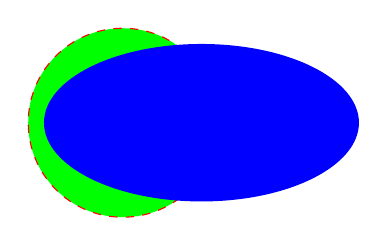
\begin{tikzpicture}
    \filldraw[color=red, fill=green, dashed] (2,0) circle (1.2);
    \fill[blue] (3,0) ellipse (2 and 1);
    \end{tikzpicture}
    
   \caption{Tikz figure}
    \label{fig:tikz1}  
\end{figure}

\begin{figure}[htbp]
\centering
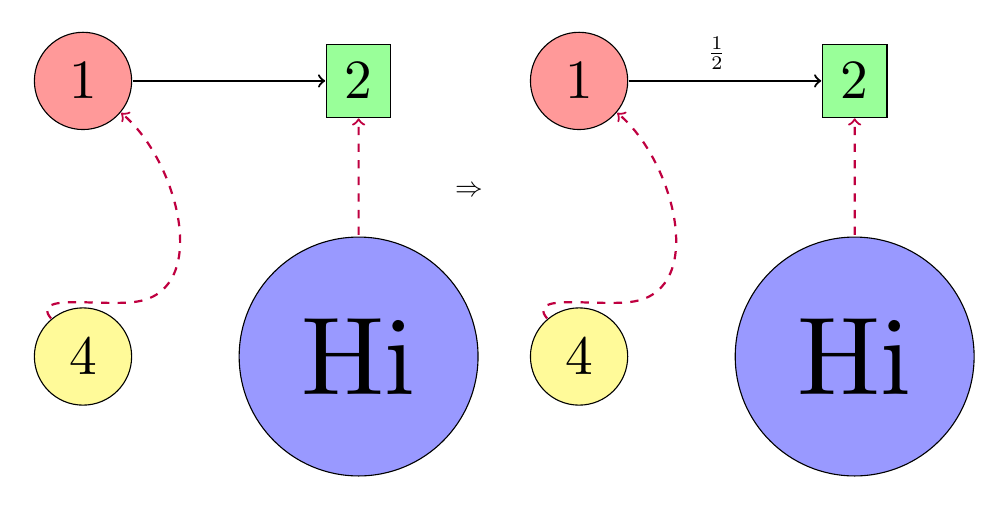
\begin{tikzpicture}[scale=.7]
\node[fill=red!40, draw=black, circle, scale=2] (1) at (0,0) {1};
\node[fill=green!40, draw=black, rectangle, scale=2] (2) at (5,0) {2};
\node[fill=blue!40, draw=black, circle, scale=4] (3) at (5,-5) {Hi};
\node[fill=yellow!40, draw=black, circle, scale=2] (4) at (0,-5) {4};
\draw[thick, ->] (1) to (2);
\draw[thick, dashed, color=purple, ->] (3) to (2);
\draw[thick, dashed, color=purple, ->] (4) to [out=130, in=190] (1,-4) to[out=10, in=-40](1);
%\node at (2.5, .5) {$\frac12$};

\node at (7, -2) {$\Rightarrow$};


\node[fill=red!40, draw=black, circle, scale=2] (1) at (0+9,0) {1};
\node[fill=green!40, draw=black, rectangle, scale=2] (2) at (5+9,0) {2};
\node[fill=blue!40, draw=black, circle, scale=4] (3) at (5+9,-5) {Hi};
\node[fill=yellow!40, draw=black, circle, scale=2] (4) at (0+9,-5) {4};
\draw[thick, ->] (1) to (2);
\draw[thick, dashed, color=purple, ->] (3) to (2);
\draw[thick, dashed, color=purple, ->] (4) to [out=130, in=190] (1+9,-4) to[out=10, in=-40](1);
\node at (2.5+9, .5) {$\frac12$};



\end{tikzpicture}
\caption{More tikz}\label{fig:tikz2}
\end{figure}

\begin{figure}[htbp]
    \centering
    \begin{tikzpicture}[scale=.6]
    \draw[ultra thick, dashed, ->] (3,0)--(6,2);
    \draw[blue, dotted] (0,0) rectangle (5,2);
    \draw[thick, dashed] (4,0)--(6,0)--(5,4)--cycle;

\begin{scope}[shift={+(3,-8)}]   
    \draw[ultra thick, dashed, ->] (3,0)--(6,2);
    \draw[blue, dotted] (0,0) rectangle (5,2);
    \draw[thick, dashed] (4,0)--(6,0)--(5,4)--cycle;
    \end{scope}
  
  \end{tikzpicture}


   \caption{Tikz figure}
    \label{fig:tikz3}  
\end{figure}

\subsection{Plotting from adjacency matrix}

\begin{figure}[htbp]
  \begin{center}
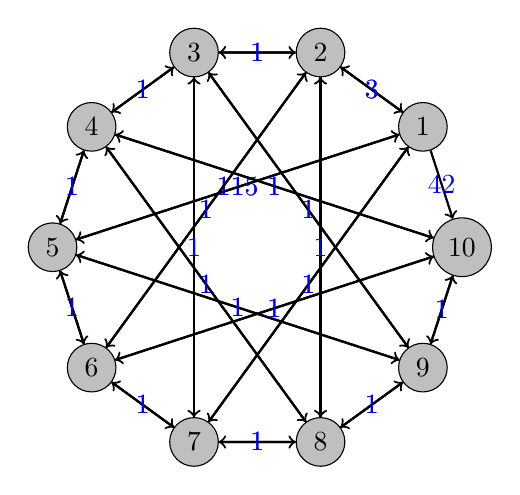
\begin{tikzpicture}[scale=2.6,vertex/.style={draw,circle,fill=gray!50}, arc/.style={draw,thick,->}]
    \foreach [count=\i] \coord in {(0.809,0.588),(0.309,0.951),(-0.309,0.951),(-0.809,0.588),(-1.,0.),(-0.809,-0.588),(-0.309,-0.951),(0.309,-0.951),(0.809,-0.588),(1.,0.)}{
        \node[vertex] (p\i) at \coord {\i};
    }

    \foreach [count=\r] \row in {{0,3,0,0,115,0,1,0,0,42},{3,0,1,0,0,1,0,1,0,0},{0,1,0,1,0,0,1,0,1,0},{0,0,1,0,1,0,0,1,0,1},{115,0,0,1,0,1,0,0,1,0},{0,1,0,0,1,0,1,0,0,1},{1,0,1,0,0,1,0,1,0,0},{0,1,0,1,0,0,1,0,1,0},{0,0,1,0,1,0,0,1,0,1},{0,0,0,1,0,1,0,0,1,0}}{
        \foreach [count=\c] \cell in \row{
            \ifnum\cell>0%
                %\draw[arc] (p\r) edge (p\c);
                \draw[arc] (p\r) edge node {\color{blue} \cell} (p\c);
            \fi
        }
    }
\end{tikzpicture}
    \caption{Generating graphs from adjacency/transition matrices.}\label{tikz:5}
  \end{center}
\end{figure}

\newpage

\section{pgfplots}

\begin{figure}[htbp]
  \begin{center}
    \begin{tikzpicture}[scale=.55]
      \begin{axis}[
          width=\linewidth, % Scale the plot to \linewidth
          %grid=major, 
          grid style={dashed,gray!30},
          xlabel=Time $t$, %X Axis $U$, % Set the labels
          ylabel=Y Axis $I$,
          x unit=hours, %\si{\volt}, % Set the respective units
          y unit=\si{\ampere},
          legend style={at={(0.5,-0.2)},anchor=north},
          x tick label style={rotate=90,anchor=east}
        ]
        \addplot 
        % add a plot from table; you select the columns by using the actual name in
        % the .csv file (on top)
        table[x=column 1,y=column 2,col sep=comma] {test.csv}; 
        \legend{Plot}
      \end{axis}
    \end{tikzpicture}
    \caption{An autogenerated plot.}\label{fig:pgfplot}
  \end{center}
\end{figure}

\newpage

\subsection{pgfplotstable}

\begin{table}[htbp]
  \begin{center}
    \caption{Autogenerated table from .csv file.}
    \label{tab:pgf}
    \pgfplotstabletypeset[
      multicolumn names, % allows to have multicolumn names
      col sep=comma, % the seperator in our .csv file
      display columns/0/.style={
        column name=$Value 1$, % name of first column
        column type={S},string type},  % use siunitx for formatting
      display columns/1/.style={
        column name=$Value 2$,
        column type={S},string type},
    display columns/2/.style={
        column name=$Value 3$,
        column type={S},string type},
      every head row/.style={
        before row={\toprule}, % have a rule at top
        after row={
            {Ampere} & \si{\volt} & \si{\tesla} \\ % the units seperated by &
            {Ampere} & {Orange $\vec{x}=0$} & {Just names} \\
            \midrule} % rule under units
            },
        every last row/.style={after row=\bottomrule}, % rule at bottom
    ]{table.csv} % filename/path to file
  \end{center}
\end{table}

%%%%%%%%%%%%%%%%%%%%%%%%%%%%%%%%%%%%%%%%%%%%%%%%%%%%%%%%%%%%%
%%%   Here references begin.

%\begin{thebibliography}{}

%\bibitem{paper1} B.~Peng, E.~Lai, A beautiful paper, {\it A Good Journal} {\bf 80} (2021), 540--542.

%\bibitem{wang2021} H.~Wang, Another beautiful paper, {\it A Good Journal} {\bf 2} (2021), 540--542.

%\end{thebibliography}

\bibliography{Ex}
\bibliographystyle{plain}
%\bibliographystyle{ieeetr}
%\bibliographystyle{apalike}
%\bibliographystyle{alpha}
%\bibliographystyle{abbrv}


\end{document}
